\section{Hoja 3: Raíces numéricas de funciones no lineales}

A continuación se va a explicar la resolución de la práctica 4. Para esta práctica se han programado en Matlab dos métodos para encontrar las raíces numéricas de funciones no lineales. El método de bisección y el método de Newton-Raphson.

\subsection{Método de bisección}
Partiendo de una función \(f(x)\) que este definida y sea continua en el intervalo \([x_1, x_2]\) tal que el signo de \(f(x_1)\) es distinto al de \(f(x_2)\) ó \(f(x_1)f(x_2) < 0\). Según el teorema de Bolzano-Weierstrass, dentro del intervalo \((x_1, x_2)\) tiene que existir al menos un valor de \(x\) tal que \(f(x) = 0\).

El método de bisección es un método iterativo en el que en cada iteración se realizan los siguientes pasos:

\begin{enumerate}
    \item Se calcula el punto medio \(m\) del intervalo como \(m = (x_1 + x_2)/2\).
    \item Si \(f(m) = 0\) entonces m es una raíz y se termina el algoritmo. Si no, se calcula el signo de \(f(m)\)
    \item En el intervalo actual \([x_1, x_2]\) se reemplaza o \(x_1\) o \(x_2\) con \(m\) tal que se siga cumpliendo que \(f(x_1)f(x_2) < 0\) para el nuevo intervalo.
    \item Se continua hasta el número de iteraciones determinado o hasta que el error sea menor que la cota predefinida.
\end{enumerate}

Usando superíndices para representar la iteración, el máximo error que se puede cometer dentro de un intervalo \([x_1^0, x_2^0]\) es \(e^1 = x_2^1 - x_1^1\) ó \(e^1 = (x_2^0 - x_2^0)/2\). Después de la \(n\) iteración, el error se puede calcular como

\[e^n = (x_2^0 - x_1^0)/2^n\]

El número de iteraciones \(n\) para que el error sea inferior a un valor \(\epsilon\) viene dado por
\[n >= \ln((x_2^0 - x_1^0) / \epsilon) / \ln(2)\]

\begin{lstlisting}[language=Matlab, caption={Algorítmo de bisección.},captionpos=b,texcl=true]
function res = Bisection(f, interval, error)
	iter = 0;
	totalIters = log((interval(2)-interval(1))/error)/log(2);

	while(iter < totalIters)
		xm = abs((interval(2)-interval(1))/2.0) + interval(1);

		if(f(xm) == 0.000)
			res = xm;
			break;
		elseif(sign(f(xm)) == sign(f(interval(2))))
			interval(2) = xm;
		elseif(sign(f(xm)) == sign(f(interval(1))))
			interval(1) = xm;
		end
		res = xm;
		iter = iter + 1;
	end
end
\end{lstlisting}

\subsection{Método de Newton-Raphson}
Dada una función de valores reales que sea continua y diferenciable, el método se basa en coger un punto inicial \((x_0^0, f(x_0^0))\) y seguir la derivada de \(f(x)\) en dicho punto en cada iteración de tal manera que el resultado de la iteración número \(n\) viene dado por la ecuación.

\[x_0^n = x_0^{n-1} - \frac{ f(x_0^{n-1}) } { f'(x_0^{n-1}) } \]

Este método puede no funcionar si alrededor del punto \(x\) o de la raíz existen máximos, mínimos o puntos de inflexión (\(f'(x) = 0\)).

El error estimado \(\epsilon\) en una iteración \(n\) se ha calculado como \(\epsilon_n = | x_n - x_{n-1} | \).

\begin{lstlisting}[language=Matlab, caption={Algorítmo de Newton-Raphson},captionpos=b,texcl=true]
function res = NewtonRaphson(f, df, startX, error)
	newX = startX;
	keepGoing = true;
	while(keepGoing)
		newX = startX - (f(startX) / df(startX));
		if ( abs(newX - startX) < error)
			keepGoing = false;
		end
		startX = newX;
	end
	res = newX;
end
\end{lstlisting}

\subsection{Resultados}

\subsubsection{Ejercicio A}

\begin{figure}[H]
    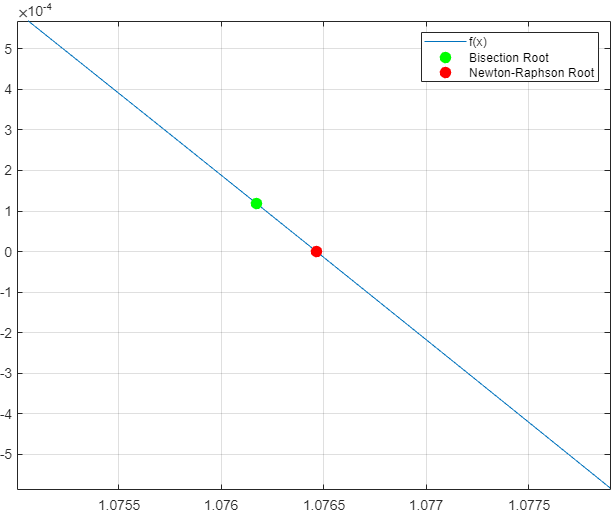
\includegraphics[width=8cm]{NumRoots/NumRoots_A}
    \centering
\end{figure}

\subsubsection{Ejercicio B}

\begin{figure}[H]
    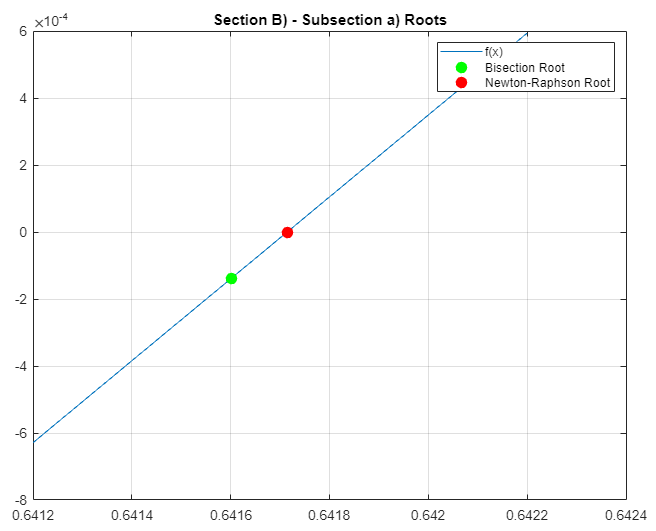
\includegraphics[width=10cm]{NumRoots/NumRoots_Ba}
    \centering
\end{figure}

\begin{figure}[H]
    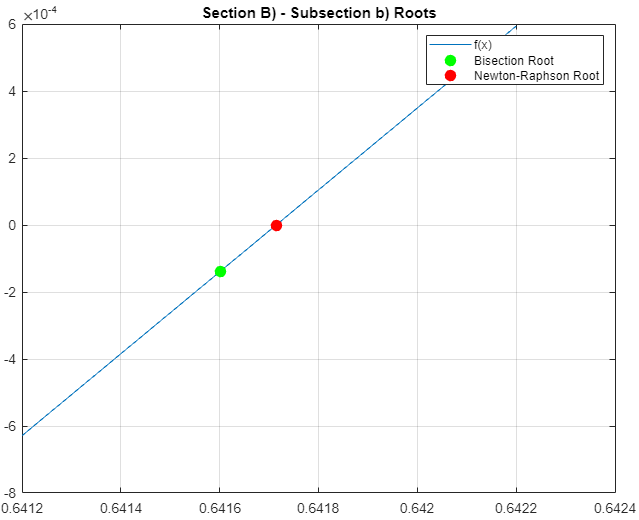
\includegraphics[width=10cm]{NumRoots/NumRoots_Bb}
    \centering
\end{figure}

\subsubsection{Ejercicio C}

\begin{figure}[H]
    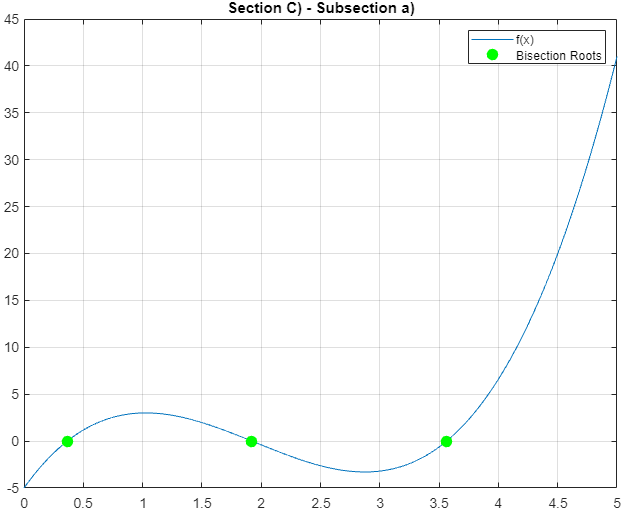
\includegraphics[width=10cm]{NumRoots/NumRoots_Ca}
    \centering
\end{figure}

\begin{figure}[H]
    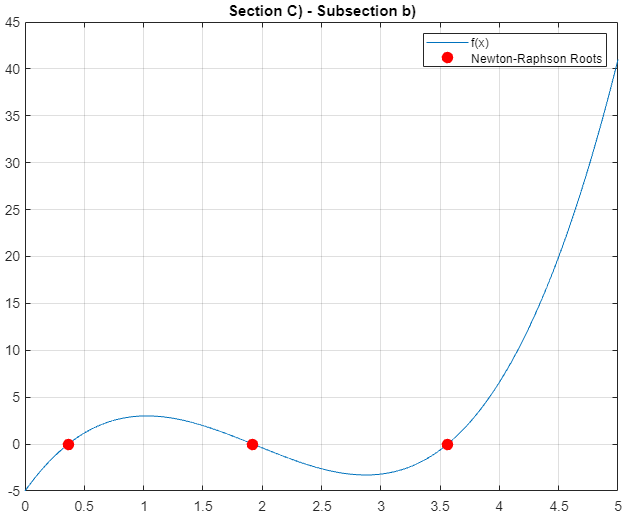
\includegraphics[width=10cm]{NumRoots/NumRoots_Cb}
    \centering
\end{figure}

\subsubsection{Ejercicio D}

\begin{figure}[H]
    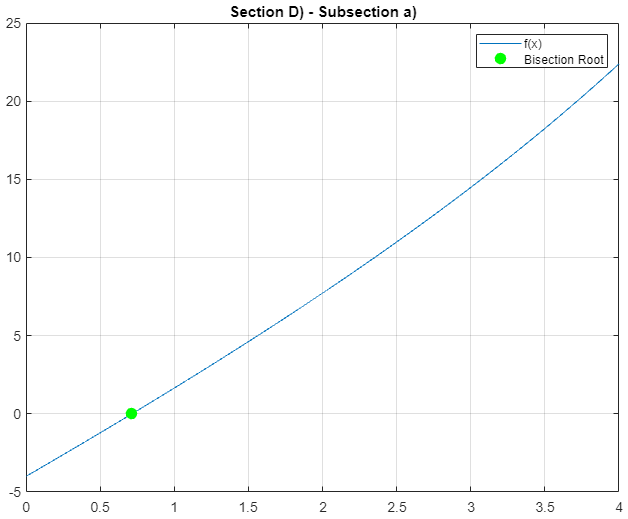
\includegraphics[width=10cm]{NumRoots/NumRoots_Da}
    \centering
\end{figure}

\begin{figure}[H]
    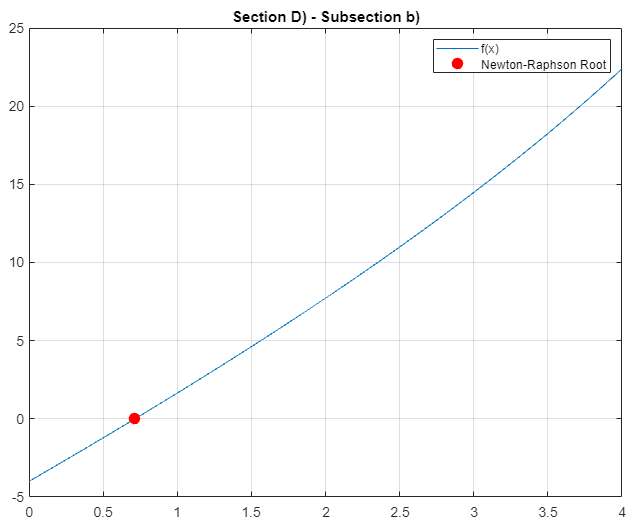
\includegraphics[width=10cm]{NumRoots/NumRoots_Db}
    \centering
\end{figure}